\documentclass[class=report, crop=false]{standalone}
\usepackage[subpreambles=true]{standalone}
\usepackage{import}

\begin{document}
We've done long range communication tests using the Yagi antenna we made. \\
\includegraphics[width=\columnwidth]{ext/radiotest.png}
\captionof{figure}{An image from the radio tests}
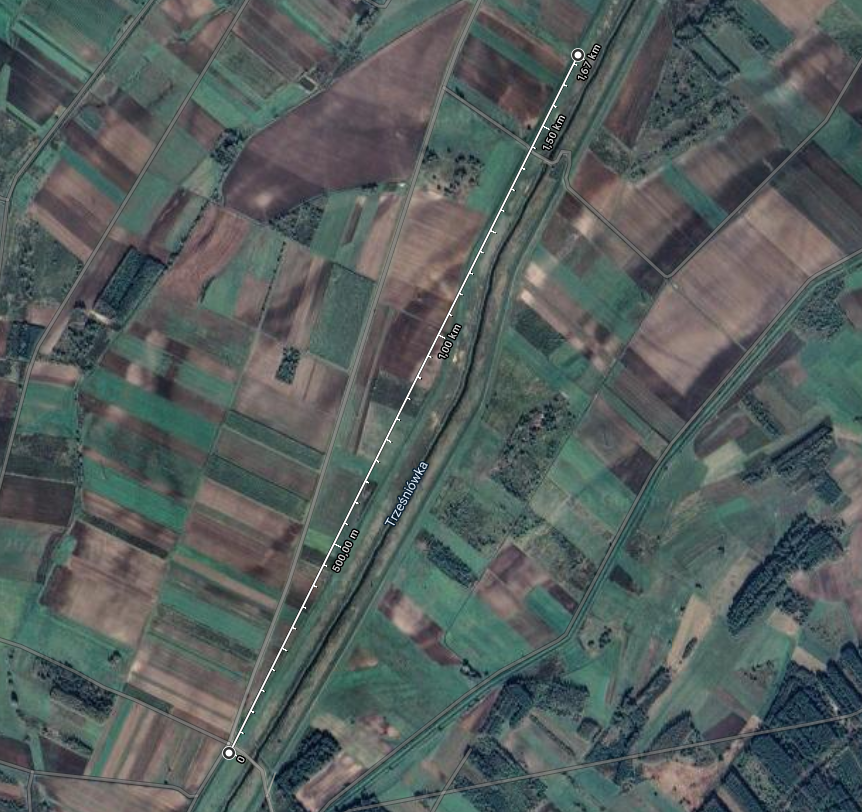
\includegraphics[width=\columnwidth]{ext/radiomap.png}
\captionof{figure}{A map of the distance between the two antennas}
Using the HC-12 SI4463 transceiver, we've concluded that the antenna has a range on the ground of around $1.7\text{km}$, which is good enough concidering that the range in the air will be better due to the lack of any terrain obstacles. 
\end{document}
